\documentclass[12pt, a4paper]{article}
\usepackage{lmodern}
%\usepackage[margin=1cm]{geometry}
\usepackage{pdflscape}
\usepackage{color}
\usepackage{footnote}
\usepackage{graphicx}
%\pagestyle{empty}
\newcommand{\cell}[2][c]{%
  \begin{tabular}[#1]{@{}c@{}}#2\end{tabular}}
\newcommand{\rowhead}[2]{\cell{\color{red}#1\\ \color{green}#2}}
\newcommand{\cont}[5]{\cell{\color{red}#1\\ \color{blue}#2\\ #3\\ #4\\ \color{green}#5}}
\newcommand{\deprecont}[5]{\cell{\color{red}#1\\ \color{blue}#2\\ #3\\ #4\\ \color{green}#5\\ \color{red}Deprecated warning}}
\newcommand{\noacc}{No accumulation}
\newcommand{\acc}{Accumulation}
\newcommand{\noconv}{No conversion}
\newcommand{\sca}{Scaling possible}
\newcommand{\nosca}{Scaling not possible}
\newcommand{\conv}{Conversion}
\newcommand{\serfal}{Service=false}
\newcommand{\sertru}{Service=true}
\newcommand{\err}{\color{red}Error}
\newcommand{\depre}{\color{red}Deprecated}
\newcommand{\follsup}{Following supports $S_{R+1}\dots S_i\dots S_N$}
\newcommand{\allsup}{All supports $S_1\dots S_i\dots S_N$}
\newcommand{\modlen}{moduleLength}
\newcommand{\modsur}{moduleSurface}
\newcommand{\nummod}{numModules}
\newcommand{\suplen}{supportLength}
\newcommand{\supsur}{supportSurface}
\newcommand{\tkl}{tkLayout}


\begin{document}
\section{Introduction to material model}
The material inside \tkl is present inside the modules (i.e. silicon
and cooling blocks),
and outside the modules (i.e. cables or cooling pipes). Is possible to
specify, in the configuration files, the material inside:
\begin{itemize}
\item modules;
\item rods (the ladders);
\item barrel's layers;
\item endcap's disks;
\item custom cylinders and disks (i.e. for the supports).
\end{itemize}
Is also possible to set material from every element:
\begin{itemize}
\item locally,
\item exiting.
\end{itemize}

\begin{figure}[h]
  \centering
  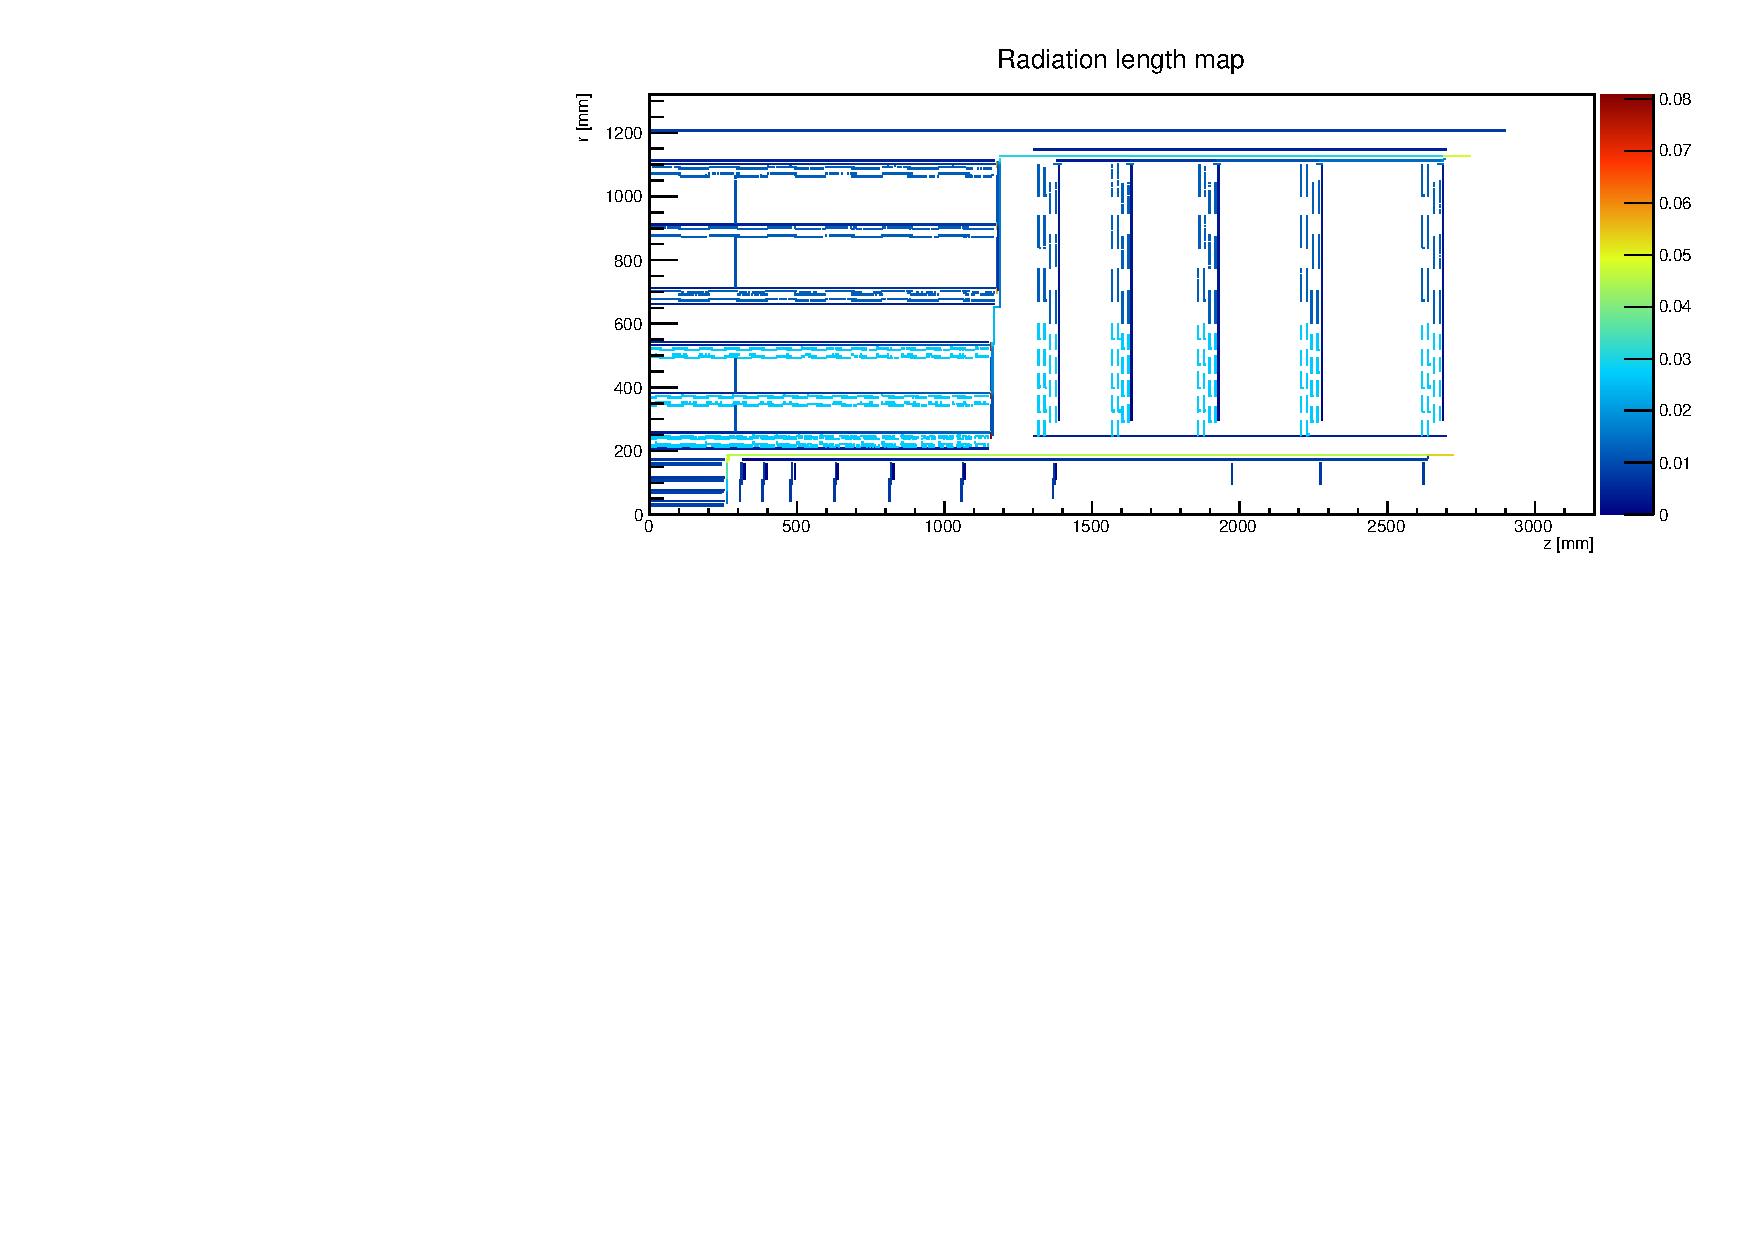
\includegraphics[width=\textwidth]{img/materialMap.pdf}  
  \caption{Material routing}
  \label{fig:materialMap}
\end{figure}

Apart from the material is possible also to define \emph{conversions}
in special points: at the end of the layers, at the end of the disks,
and in custom positon along the way.

In figure~\ref{fig:materialMap}
is visible the material for the modules and the \emph{sections} for
the routing of the material, section~\ref{sec:userManual} deal with
the description in detail of how to build the configuration files and
how the material is distributed, from an user point of view.

The material \emph{routing algorithm} builds automatically all the necessary structures for
keeping all the materials that not belongs to the modules. It builds
\emph{sections} on top of the layers, and on the right of the disks,
then connect those sections for each barrel and endcap, then connect
barrels and endcaps with the cable exit point (upper right point of
tracker). Section~\ref{sec:developerManual} deal with the description
in detail of the routing algorithm from a developer point of view.




\section{User manual}\label{sec:userManual}
\subsection{Material routing effects}
The first column is where the material is defined and if is defined
with \emph{service} true or false. The other columns are the different
effect regarding the unit of measure of the material, for each cell:
the first field is the destination volume; the second is the amount of
material in grams; the third specify if the material is accumulating
along the layer/disk; the fourth specify if the material is converted
after the layer/disk or only stay in the layer/disk; the fifth if is
possible or not to set the scaling on channels.
\begin{landscape}
  \begin{savenotes}
    \begin{center}
      \fontsize{7pt}{8.3}\selectfont
      \begin{tabular}{|c||c|c|c|}
        \hline
        & \color{green}Unit=$g/m$ & \color{green}Unit=$mm$ & \color{green}Unit=$g$\\
        \hline\hline
        \rowhead{Module}{\serfal} & \cont{Module}{$\times \modlen$}{\noacc}{\noconv}{\sca}& \cont{Module}{$\times \modsur\times \rho$ (sensor surface)}{\noacc}{\noconv}{\sca}& \cont{Module}{$\times 1$}{\noacc}{\noconv}{\sca}\\
        \hline
        \rowhead{Module in ring $R$\footnote{of $N$ rings}}{\sertru\footnote{\label{sertrunote}may be converted by station}} & \cont{\follsup}{$\times \nummod_R \times \suplen_i$}{\acc}{\conv (1:1 by default, with warning)}{\sca} & \deprecont{\follsup}{$\times \nummod_R \times \supsur_i \times \rho$}{\acc}{\conv  (1:1 by default, with warning)}{\sca} & \err \\
        \hline
        \rowhead{Rod (barrel\footnote{line of one module per ring with same $\phi$})}{\serfal} & \cont{\allsup}{$\times \nummod_1 \times \suplen_i$}{\noacc}{\noconv}{\nosca} & \cont{\allsup}{$\times \supsur_i \times \rho$}{\noacc}{\noconv}{\nosca} & \cont{\allsup}{$\times \nummod_1 \times \frac{\suplen_i}{\sum_{j=1}^N\suplen_j}$}{\noacc}{\noconv}{\nosca} \\
        \hline
        \rowhead{Rod (barrel)}{\sertru\textsuperscript{\ref{sertrunote}}} & \cont{\allsup}{$\times \nummod_1 \times \suplen_i$}{\noacc}{\conv}{\nosca} & \deprecont{\allsup}{$\times \supsur_i \times \rho$}{\noacc}{\conv}{\nosca} & \err \\
        \hline
        \rowhead{Layer/Disk}{\serfal} & \cont{\allsup}{$\times \suplen_i$}{\noacc}{\noconv}{\nosca} & \cont{\allsup}{$\times \supsur_i \times \rho$}{\noacc}{\noconv}{\nosca} & \cont{\allsup}{$\times \frac{\suplen_i}{\sum_{j=1}^N\suplen_j}$}{\noacc}{\noconv}{\nosca} \\
        \hline
        \rowhead{Layer/Disk}{\sertru\textsuperscript{\ref{sertrunote}}} & \cont{\allsup}{$\times \suplen_i$}{\noacc}{\conv}{\nosca} & \deprecont{\allsup}{$\times \supsur_i \times \rho$}{\noacc}{\conv}{\nosca} & \err \\
        \hline
      \end{tabular}
    \end{center}
    \begin{center}
      \tiny
      \begin{tabular}{|c|c|c|c|}
        \hline
        & Modules & Cylind. service sections & disk service section \\
        \hline
        Length & Local $y$ & $\Delta z$ & $\Delta r$ \\
        \hline
        Surface & Sensor surface & $2\pi r \Delta z$ & $\pi({r_2}^2 - {r_1}^2)$ \\
        \hline
      \end{tabular}
    \end{center}
  \end{savenotes}
\end{landscape}



\section{Developer manual}\label{sec:developerManual}

\subsection{General algorithm description}






\subsection{Classes description}

\subsubsection{namespace insur}

\begin{itemize}

\item \textbf{MaterialBudget}\\
This class integrates information from a \emph{Tracker} and an \emph{InactiveSurface} instance with a collection of \emph{ModuleCap} instances to provide the full material budget of a tracker.\\
Its main function accepts an instance of a material calculator as an input parameter in order to use that calculator's more specialised functions to assign mixtures of materials to the different categories of volumes in the tracker geometry. Afterwards, each individual volume is ready to calculate its total mass, its radiation length and its interaction length, which is also taken care of by the calculator class. A material budget that has been filled in this way can then be passed on to be analysed by an instance of an \emph{Analyzer} class.

\item \textbf{MaterialProperties}\\
This is the base class for collections of properties related to the material budget.\\
It encapsulates the main parameters of interest, namely the overall density, radiation length and interaction length of a tracker element, as well as the influence of the materials that make up this building block. Access functions are provided where appropriate. But unless the object is cloned the overall parameters should typically be calculated from a list of materials and their properties rather than set explicitly. Some of the access functions for individual materials may throw exceptions if the requested material does not appear on the list.

\item \textbf{MaterialTable} \\
Essentially, this is a collection class for \emph{MaterialRow} instances.\\
It provides access functions for individual entries and a couple of bookkeeping calls.\\
The access functions may trow exceptions if an entry doesn't exist or if an index is out of range.

\item \textbf{BaseMaterial}
\item \textbf{MaterialTable2}
\item \textbf{ElementaryMaterial : public BaseMaterial}
\item \textbf{CompositeMaterial : public BaseMaterial}

\item \textbf{InactiveElement : public MaterialProperties}\\
This is the base class for the elements that make up the inactive surfaces.\\
Since all inactive elements are simplified to tube shapes in the geometrical model, the geometry parameters have been packed into the base class. All of these parameters apply to descendants of a different shape as well, though, because they describe relations between the object and the origin, not between points within the object.

\item \textbf{InactiveRing : public InactiveElement}\\
The only thing that this class adds to its parent is a check that it is a ring rather than a tube.

\item \textbf{InactiveSurfaces}\\
This is the top-level container class  for the inactive surfaces.\\
It contains lists of all subgroups of inactive volumes: the services list and the supporting parts list.\\
It provides access functions to them or their individual elements that typically copy a new element to its place at the end of the vector or return a reference to a requested element. It also stores the type of configuration (UP or DOWN) in a boolean flag. Some of the access functions to individual elements may throw an exception if the requested index is out of range.

\item \textbf{InactiveTube : public InactiveElement}\\
The only thing that this class adds to its parent is a check that it is a tube rather than a ring.

\item \textbf{MatCalc}\\
This class provides the core material assignment algorithm for a given tracker geometry.\\
Once its internal data structures have been initialised from the material config file by the \emph{MatParser} class, it uses that information, combined with the geometry and position of an individual tracker element, to set the local and exiting materials vector that element before getting it to calculate its overall mass, its radiation length and its interaction length. The tracker geometry is ready for further study afterwards. Some of the access functions for various internal list elements may return an exception if the requested element does not exist on the list.

\end{itemize}



\subsubsection{namespace material}

\begin{itemize}

\item \textbf{MaterialObject : public PropertyObject}
\item \textbf{MaterialObject::ReferenceSensor : public PropertyObject}
\item \textbf{MaterialObject::MaterialObjectKey}
\item \textbf{MaterialObject::Element : public PropertyObject}
\item \textbf{MaterialObject::Component : public PropertyObject}
\item \textbf{MaterialObject::Materials : public PropertyObject}
\item \textbf{MaterialSection : public MaterialObject}
\item \textbf{MaterialStation : public MaterialSection}
\item \textbf{MaterialTab : public MaterialTabType}

\item \textbf{Materialway}\\
Represents a track where the materials are routed from the modules to the appropriate end.\\ 
The materialway is make up from single elements \emph{Element}, every element pointing to the possible single next element. Every module is linked to a materialway element where it puts its materials to be routed, the material is then deposited on the element and forwarded to the next element, passing through the chain from an element to the subsequent one until the material reaches its designated end.\\ 
Every materialway element can perform some transformation on the routed material before it is forwarded to the next element.

\item \textbf{Materialway::RodSectionsStation}

\item \textbf{Materialway::Section}\\
Represents a single element of the materialway.

\item \textbf{Materialway::Station : public Materialway::Section}

\item \textbf{Materialway::Boundary}\\
Represents a boundary where the services are routed around.

\item \textbf{Materialway::OuterUsher}\\
This is the core of the functionality that builds sections across boundaries starting from a point and ending to another section or to the upper right angle.

\item \textbf{Materialway::InnerUsher}\\
Builds the internal sections of a boundary.

\item \textbf{Materialway::ModuleUsher}\\
Adds materials to the modules.

\item \textbf{ConversionStation : public MaterialObject}
\item \textbf{ConversionStation::Inoutput : public PropertyObject}
\item \textbf{ConversionStation::Conversion : public PropertyObject}
\item \textbf{WeightDistributionGrid : public WeightDistributionGridMapType}

\end{itemize}



\end{document}


